% samyama.tex — arxiv submission (cs.DB)
% Single-column article class, standard for cs.DB arxiv submissions
\documentclass[11pt]{article}

% --- Packages ---
\usepackage[utf8]{inputenc}
\usepackage[T1]{fontenc}
\usepackage{lmodern}
\usepackage[margin=1in]{geometry}
\usepackage{amsmath,amssymb}
\usepackage{graphicx}
\usepackage{booktabs}
\usepackage{hyperref}
\usepackage{xcolor}
\usepackage{listings}
\usepackage{natbib}
\usepackage{float}
\usepackage{enumitem}
\usepackage{url}
\usepackage{microtype}

% --- Hyperref setup ---
\hypersetup{
  colorlinks=true,
  linkcolor=blue!70!black,
  citecolor=blue!70!black,
  urlcolor=blue!70!black
}

% --- Listings setup for Cypher ---
\lstdefinelanguage{Cypher}{
  keywords={MATCH, RETURN, WHERE, CREATE, DELETE, SET, REMOVE, MERGE, WITH, UNWIND, UNION, ORDER, BY, SKIP, LIMIT, EXPLAIN, PROFILE, CALL, YIELD, AS, DISTINCT, OPTIONAL, AND, OR, NOT, IN, IS, NULL, TRUE, FALSE, EXISTS, CASE, WHEN, THEN, ELSE, END, DROP, SHOW, INDEX, INDEXES, CONSTRAINTS, ON},
  sensitive=false,
  morestring=[b]',
  morestring=[b]",
  morecomment=[l]{//},
}

\lstset{
  language=Cypher,
  basicstyle=\ttfamily\small,
  keywordstyle=\bfseries\color{blue!70!black},
  stringstyle=\color{red!70!black},
  commentstyle=\itshape\color{gray},
  breaklines=true,
  frame=single,
  framesep=3pt,
  xleftmargin=6pt,
  xrightmargin=6pt,
  aboveskip=8pt,
  belowskip=8pt
}

% --- Title ---
\title{Samyama: A Unified Graph-Vector Database with In-Database Optimization,\\Agentic Enrichment, and Hardware Acceleration}

\author{
  Madhulatha Mandarapu\thanks{madhulatha@samyama.ai, ORCID: \url{https://orcid.org/0009-0005-2837-6725}} \and
  Sandeep Kunkunuru\thanks{sandeep@samyama.ai, ORCID: \url{https://orcid.org/0000-0002-8886-1846}}
}
\date{%
  VaidhyaMegha Private Limited, India\\[2pt]
  \url{https://samyama.ai/}\\[8pt]
  March 2026 \quad|\quad v0.6.0
}

\begin{document}
\maketitle

% ============================================================
% ABSTRACT
% ============================================================
\begin{abstract}
Modern data architectures are fragmented across graph databases, vector stores, analytics engines, and optimization solvers, resulting in complex ETL pipelines and synchronization overhead. We present Samyama, a high-performance graph-vector database written in Rust that unifies these workloads into a single engine. Samyama combines a RocksDB-backed persistent store with a versioned-arena MVCC model, a vectorized query executor with 35 physical operators, a cost-based query planner with plan enumeration and predicate pushdown, a dedicated CSR-based analytics engine, and native RDF/SPARQL support. The system integrates 22 metaheuristic optimization solvers directly into its query language, implements HNSW vector indexing with Graph RAG capabilities, and introduces Agentic Enrichment for autonomous graph expansion via LLMs. The Enterprise Edition adds GPU acceleration via wgpu, production-grade observability, point-in-time recovery, and hardened high availability with HTTP/2 Raft transport.

Our evaluation on commodity hardware (Mac Mini M4, 16\,GB RAM) demonstrates: ingestion at 255K nodes/s (CPU) and 412K nodes/s (GPU-accelerated); 115K Cypher queries/sec at 1M nodes; 4.0--4.7$\times$ latency reduction from late materialization on multi-hop traversals; 8.2$\times$ GPU PageRank speedup at 1M nodes; and 100\% LDBC Graphalytics validation (28/28 tests). These results demonstrate that a unified graph-vector-optimization engine can achieve competitive performance on commodity hardware while maintaining Rust's memory safety guarantees.
\end{abstract}

\noindent\textbf{Keywords:} Graph Databases, Vector Search, Distributed Systems, Metaheuristic Optimization, Rust, GPU Acceleration, Agentic AI, RDF, LDBC.

% ============================================================
% 1. INTRODUCTION
% ============================================================
\section{Introduction}

The rise of Large Language Models (LLMs) has popularized Retrieval-Augmented Generation (RAG), creating demand for systems that handle both relational structure (graphs) and semantic similarity (vectors). Simultaneously, industrial applications increasingly require in-database optimization for resource allocation, scheduling, and supply chain management. Existing solutions force developers to compose architectures from disparate systems---Neo4j for graphs, Pinecone for vectors, Spark for analytics, and Python/Gurobi for optimization---incurring data movement overhead and operational complexity.

Samyama (Sanskrit for ``Integration'') is designed as an AI-native database that treats graphs, vectors, and optimization as first-class citizens within a single memory-safe engine. We organize our contributions into two categories:

\paragraph{Primary research contributions:}
\begin{enumerate}[leftmargin=*]
  \item \textbf{Late materialization for graphs}: \texttt{NodeRef}-based lazy property resolution~\citep{abadi2008column} achieving 4.0--4.7$\times$ traversal speedup (\S\ref{sec:query-engine}, \S\ref{sec:late-mat-eval}).
  \item \textbf{In-database metaheuristic optimization}: 22 solvers accessible directly via Cypher procedures, eliminating ETL overhead for graph-native optimization (\S\ref{sec:optimization}).
  \item \textbf{Agentic Enrichment (GAK)}: Autonomous graph expansion using LLM tool-calling, transforming the database from a passive store into a self-evolving knowledge graph (\S\ref{sec:agentic}).
\end{enumerate}

\paragraph{Engineering contributions:}
\begin{enumerate}[leftmargin=*,resume]
  \item \textbf{Unified engine}: Property graph + vector search + analytics + optimization in one binary.
  \item \textbf{Cost-based query planner}: Plan enumeration, predicate pushdown, early LIMIT propagation, plan cache, and join reordering (\S\ref{sec:query-engine}).
  \item \textbf{Cross-platform GPU acceleration}: wgpu-based compute shaders for graph algorithms and PCA.
  \item \textbf{SDK ecosystem}: Rust, Python (PyO3), TypeScript SDKs with embedded and remote access patterns.
  \item \textbf{RDF interoperability}: Native RDF data model~\citep{w3c2014rdf} with Turtle/N-Triples/RDF-XML serialization.
  \item \textbf{Industry validation}: 100\% LDBC Graphalytics~\citep{iosup2016ldbc} pass rate (28/28 tests).
\end{enumerate}

This paper focuses its evaluation on the three primary research contributions: late materialization (\S\ref{sec:late-mat-eval}), in-database optimization (\S\ref{sec:opt-eval}), and agentic enrichment (\S\ref{sec:gak-eval}). The remaining system features are described for architectural completeness.

% ============================================================
% 2. SYSTEM ARCHITECTURE
% ============================================================
\section{System Architecture}

Samyama is built on a modern Rust stack for memory safety and zero-cost abstractions. Figure~\ref{fig:architecture} illustrates the overall system architecture.

\begin{figure}[t]
  \centering
  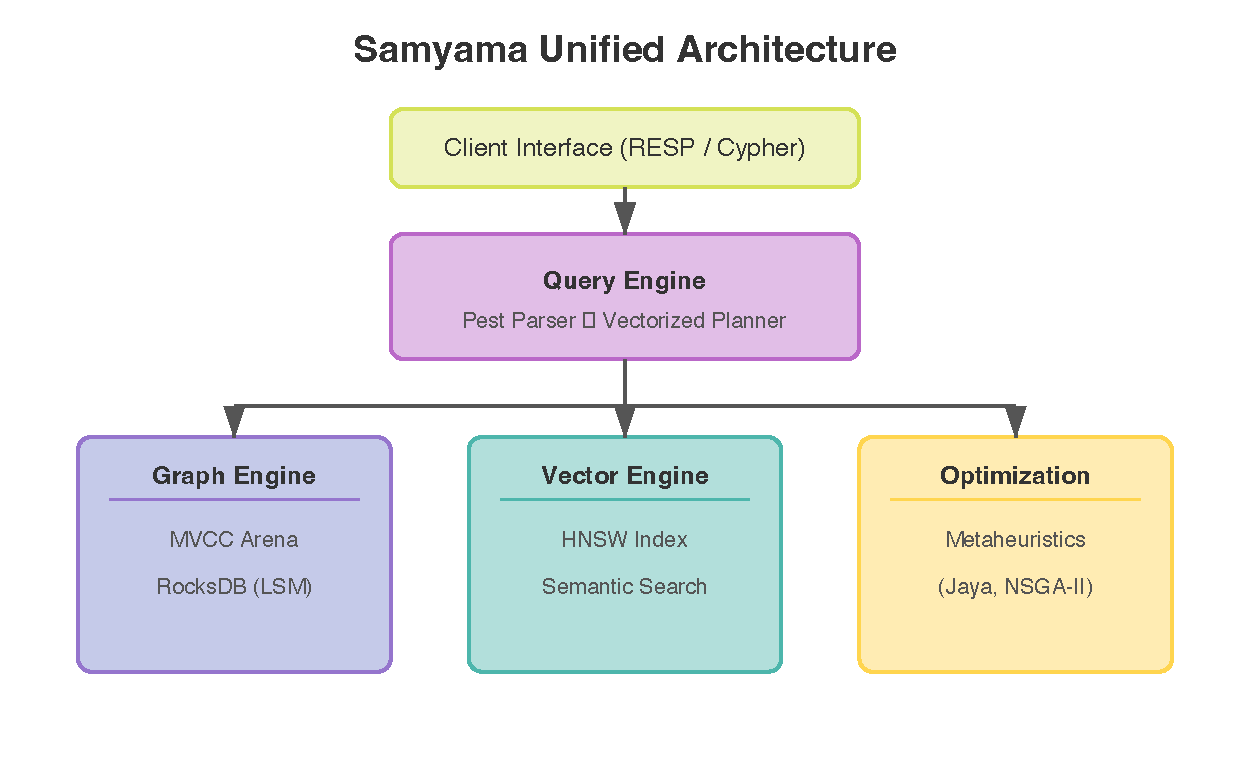
\includegraphics[width=\linewidth]{figures/architecture.pdf}
  \caption{Samyama system architecture. OpenCypher queries flow through the cost-based planner and vectorized executor to the RocksDB/MVCC storage layer.}
  \label{fig:architecture}
\end{figure}

\subsection{Storage Engine}

We utilize \textbf{RocksDB} for persistence, employing a tiered Log-Structured Merge (LSM) tree~\citep{oneil1996lsm} with LZ4 and Zstd compression. Data isolation is achieved through \textbf{Column Families}, providing independent compaction, backup, and key namespaces per tenant.

Key design: \texttt{NodeId} and \texttt{EdgeId} are direct \texttt{u64} indices into contiguous arena storage (\texttt{Vec<Vec<T>>}), eliminating hash lookups and providing $O(1)$ access with cache-friendly memory layout.

\subsection{Memory Management \& MVCC}

Samyama implements \textbf{Multi-Version Concurrency Control (MVCC)}~\citep{bernstein1981mvcc} within a versioned-arena structure. The inner vector stores version history, enabling \textbf{Snapshot Isolation} without read locks. Write atomicity is guaranteed via RocksDB \texttt{WriteBatch} + WAL~\citep{mohan1992aries}.

ACID guarantees: Atomicity (WriteBatch), Consistency (schema validation + Raft quorum), Isolation (per-query via RwLock, MVCC foundation), Durability (RocksDB + Raft replication).

\subsection{Query \& Execution Engine}
\label{sec:query-engine}

Samyama supports ${\sim}90\%$ of \textbf{OpenCypher}. Queries are parsed via a PEG parser~\citep{ford2004peg} (\texttt{pest} crate with atomic keyword rules for word boundary enforcement) and executed using a hybrid \textbf{Volcano--Vectorized} model~\citep{graefe1994volcano} with batch size 1,024.

The engine implements \textbf{35 physical operators} organized across scan, traversal, filter, join, aggregation, sort, write, index, and specialized categories. Key v0.6.0 additions include:

\begin{itemize}[leftmargin=*]
  \item \textbf{Cost-based planner}: Plan enumeration over candidate plans using a \texttt{GraphCatalog} with triple-level statistics (\texttt{TriplePattern} $\to$ \texttt{TripleStats}). The planner selects the lowest-cost plan based on multiplicative cardinality estimates.
  \item \textbf{Predicate pushdown}: Filter predicates are pushed below Expand operators when they reference only the source variable, reducing intermediate cardinality.
  \item \textbf{ExpandInto operator}: When both endpoints of an edge pattern are already bound, \texttt{ExpandIntoOperator} checks edge existence via binary search on sorted adjacency lists ($O(\log d)$), avoiding full fan-out.
  \item \textbf{Plan cache}: Compiled physical plans are cached by query AST hash, eliminating planning overhead for repeated queries.
  \item \textbf{Join reordering}: Multi-pattern MATCH clauses are reordered by estimated cardinality to minimize intermediate result sizes.
  \item \textbf{Parameterized queries}: \texttt{\$param} syntax for safe query reuse without re-parsing.
  \item \textbf{PROFILE}: Runtime statistics (rows produced, time per operator) for query performance analysis.
\end{itemize}

\paragraph{Late Materialization (ADR-012).}
Scan operators produce \texttt{Value::NodeRef(id)} instead of full node clones. Properties are resolved on-demand via the \texttt{ColumnStore} at the final \texttt{ProjectOperator}, reducing memory bandwidth by 4--5$\times$. This technique adapts the columnar late materialization strategy described in~\citet{abadi2008column} to a graph context.

\subsection{RDF \& SPARQL}

Samyama provides native RDF~\citep{w3c2014rdf} support via the \texttt{oxrdf} crate: an in-memory triple store with SPO/POS/OSP indices for $O(1)$ pattern matching; serialization in Turtle, N-Triples, RDF/XML (read/write) and JSON-LD (write); pre-loaded namespace prefixes (rdf, rdfs, xsd, owl, foaf, dc); and SPARQL~\citep{w3c2013sparql} parser infrastructure via \texttt{spargebra} with query execution in development.

\subsection{Indexing \& Constraints}
\label{sec:indexing}

Samyama v0.6.0 introduces composite indexes, unique constraints, and index management commands:

\begin{itemize}[leftmargin=*]
  \item \textbf{Composite indexes}: Multi-property indexes for efficient compound lookups (e.g., \texttt{CREATE INDEX ON :Person(name, age)}).
  \item \textbf{Unique constraints}: Schema-level uniqueness enforcement with automatic index backing.
  \item \textbf{AND-chain index selection}: The planner selects the most selective index when multiple predicates are joined by AND.
  \item \textbf{Management}: \texttt{DROP INDEX}, \texttt{SHOW INDEXES}, \texttt{SHOW CONSTRAINTS} for operational visibility.
\end{itemize}

% ============================================================
% 3. HIGH-PERFORMANCE ANALYTICS
% ============================================================
\section{High-Performance Analytics}

\subsection{CSR Projection}

For global graph analytics, Samyama projects the relevant subgraph into a \textbf{Compressed Sparse Row (CSR)} format (\texttt{GraphView}). Three contiguous arrays (\texttt{out\_offsets}, \texttt{out\_targets}, \texttt{weights}) enable sequential memory access with near-perfect CPU prefetch accuracy and zero-lock parallelism via \texttt{rayon}. Figure~\ref{fig:csr} illustrates the CSR data layout.

\begin{figure}[t]
  \centering
  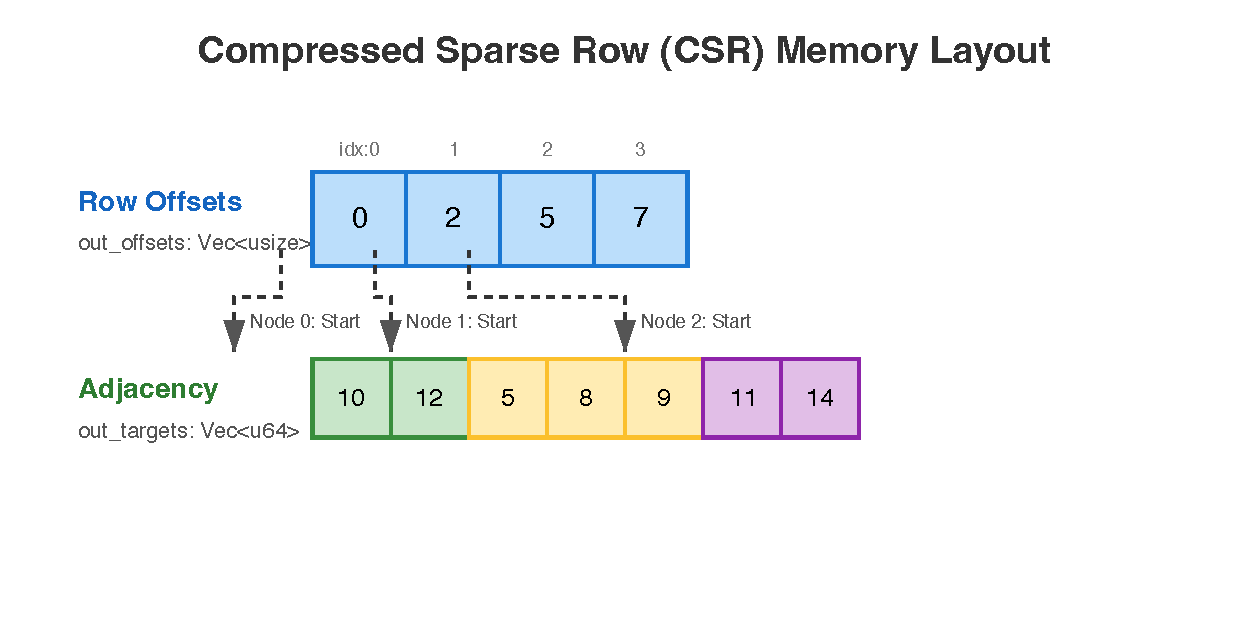
\includegraphics[width=0.85\linewidth]{figures/csr_layout.pdf}
  \caption{CSR data layout. \texttt{out\_offsets} and \texttt{out\_targets} arrays enable cache-efficient sequential traversal.}
  \label{fig:csr}
\end{figure}

\subsection{Algorithm Library}

The \texttt{samyama-graph-algorithms} crate provides 14 algorithms across five categories (Table~\ref{tab:algorithms}).

\begin{table}[t]
  \centering
  \caption{Graph algorithm library.}
  \label{tab:algorithms}
  \begin{tabular}{@{}lp{10cm}@{}}
    \toprule
    \textbf{Category} & \textbf{Algorithms} \\
    \midrule
    Centrality   & PageRank~\citep{page1999pagerank} (with dangling redistribution), LCC~\citep{watts1998smallworld} \\
    Community    & WCC (Union-Find), SCC (Tarjan~\citep{tarjan1972dfs}), CDLP~\citep{raghavan2007cdlp}, Triangle Counting \\
    Pathfinding  & BFS, Dijkstra~\citep{dijkstra1959note}, BFS All Shortest Paths \\
    Network Flow & Edmonds-Karp~\citep{edmonds1972maxflow} (Max Flow), Prim's MST \\
    Statistical  & PCA (Randomized SVD~\citep{halko2011randomized} + Power Iteration) \\
    \bottomrule
  \end{tabular}
\end{table}

PCA implements the Halko--Martinsson--Tropp algorithm~\citep{halko2011randomized} for Randomized SVD with $O(n \cdot d \cdot k)$ complexity, auto-selecting over Power Iteration when $n > 500$ nodes.

% ============================================================
% 4. IN-DATABASE OPTIMIZATION
% ============================================================
\section{In-Database Optimization}
\label{sec:optimization}

Unique to Samyama is the integration of \textbf{22 metaheuristic optimization solvers} in the \texttt{samyama-optimization} crate, accessible directly through Cypher procedures:

\begin{minipage}{\linewidth}
\begin{lstlisting}
CALL algo.or.solve({
  algorithm: 'NSGA2',
  label: 'Generator',
  objectives: ['cost', 'emissions'],
  constraints: [{ property: 'load', max: 500.0 }],
  population_size: 100
}) YIELD pareto_front
\end{lstlisting}
\end{minipage}

Solvers include: Jaya~\citep{rao2016jaya}, QOJAYA, Rao (1--3)~\citep{rao2020rao}, TLBO~\citep{rao2011tlbo}, ITLBO, GOTLBO, PSO~\citep{kennedy1995pso}, DE~\citep{storn1997de}, GA~\citep{holland1975ga}, GWO~\citep{mirjalili2014gwo}, ABC~\citep{karaboga2005abc}, BAT~\citep{yang2010bat}, Cuckoo Search~\citep{yang2009cuckoo}, Firefly~\citep{yang2009firefly}, FPA~\citep{yang2012fpa}, GSA~\citep{rashedi2009gsa}, SA~\citep{kirkpatrick1983sa}, HS~\citep{geem2001hs}, BMR, BWR, NSGA-II~\citep{deb2002nsga2}, and MOTLBO. Multi-objective solvers implement the \textbf{Constrained Dominance Principle} for feasibility-first Pareto optimization. All solvers leverage Rayon for parallel fitness evaluation across CPU cores.

\subsection{In-Database Optimization Evaluation}
\label{sec:opt-eval}

A key advantage of in-database optimization is the elimination of ETL overhead. In a conventional workflow, graph data must be extracted to an external solver (e.g., Python/Gurobi), transformed into the solver's input format, optimized, and the results imported back. For a supply chain graph with $N$ nodes and $M$ edges, the data extraction and serialization step alone incurs $O(N + M)$ I/O overhead. Samyama's in-database solvers operate directly on the graph store, avoiding this round-trip entirely.

Figure~\ref{fig:pareto} shows a representative Pareto front from NSGA-II applied to a supply chain scenario with two objectives (cost vs.\ emissions) and capacity constraints, demonstrating that the in-database solver produces well-distributed non-dominated solutions without external tooling.

\begin{figure}[H]
  \centering
  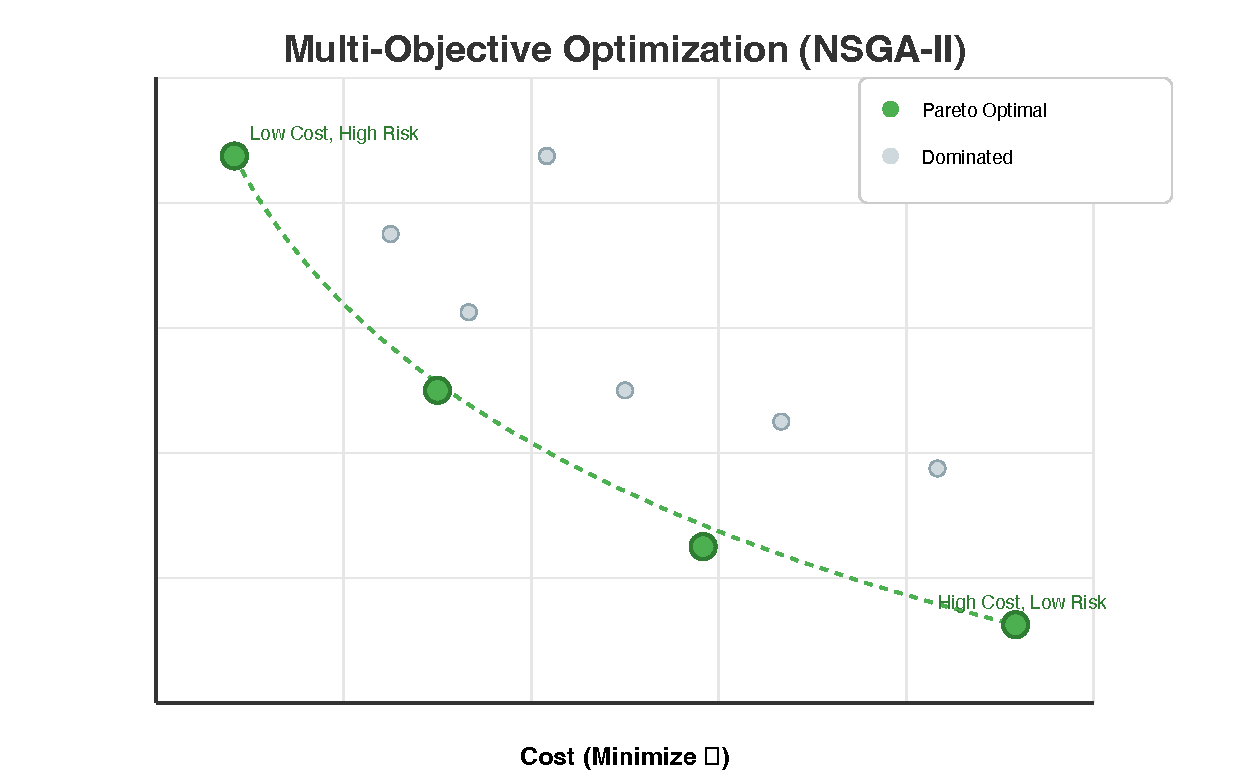
\includegraphics[width=0.8\linewidth]{figures/pareto_front.pdf}
  \caption{NSGA-II Pareto front for a supply chain optimization scenario (cost vs.\ emissions). Solutions are produced entirely in-database without external solver tooling.}
  \label{fig:pareto}
\end{figure}

We note that a detailed convergence comparison against established solvers (e.g., Gurobi, CPLEX) on standard benchmark functions is deferred to future work. The primary contribution here is the architectural integration---making graph-native optimization a first-class query primitive---rather than claiming superiority over specialized mathematical programming solvers.

% ============================================================
% 5. AI & AGENTIC ENRICHMENT
% ============================================================
\section{AI \& Agentic Enrichment}

\subsection{Vector Search}

Samyama implements \textbf{HNSW}~\citep{malkov2020hnsw} indexing (via \texttt{hnsw\_rs}) for millisecond-speed approximate nearest neighbor search with Cosine, L2, and Dot Product metrics. The \texttt{VectorSearchOperator} integrates with standard graph operators for \textbf{Graph RAG}---combining vector retrieval with graph traversal in a single query execution.

\subsection{Agentic Enrichment (GAK)}
\label{sec:agentic}

We introduce \textbf{Generation-Augmented Knowledge (GAK)}: an autonomous loop where the database uses LLMs to fetch and create missing data. The \texttt{AgentRuntime} manages tool-calling agents (\texttt{WebSearchTool}, \texttt{NLQClient}) that discover information and generate Cypher \texttt{CREATE} commands, transforming the database from a passive store to a self-evolving knowledge graph. Safety validation includes schema checking, destructive query rejection, and rate limiting. Figure~\ref{fig:agentic} illustrates the agentic enrichment loop.

\begin{figure}[t]
  \centering
  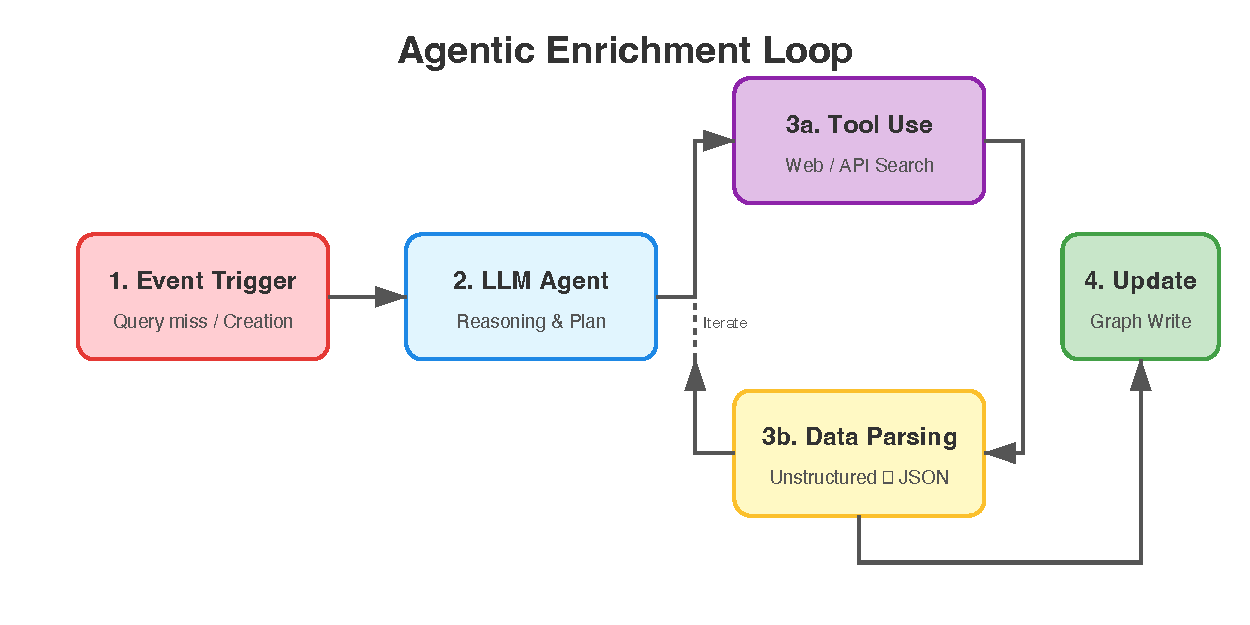
\includegraphics[width=0.85\linewidth]{figures/agentic_loop.pdf}
  \caption{Agentic Enrichment (GAK) loop. An event-driven trigger invokes LLM tool-calling to discover and create graph data autonomously.}
  \label{fig:agentic}
\end{figure}

\subsection{Natural Language Query (NLQ)}

The \texttt{NLQPipeline} converts natural language questions to Cypher via LLM providers (OpenAI, Gemini, Ollama, Claude). Generated queries undergo safety validation (\texttt{is\_safe\_query()}) before execution.

\subsection{Agentic Enrichment Evaluation}
\label{sec:gak-eval}

While the GAK architecture is fully implemented and demonstrated across multiple domain examples (pharmaceutical, financial, security), a rigorous quantitative evaluation requires addressing several challenges:

\begin{itemize}[leftmargin=*]
  \item \textbf{Hallucination risk}: LLM-generated triples may contain factual errors. Precision depends on the underlying LLM, prompt design, and domain specificity.
  \item \textbf{Schema drift}: Autonomous enrichment may introduce labels or relationship types not in the original schema, requiring schema validation guards.
  \item \textbf{Cost at scale}: Each enrichment cycle incurs LLM API costs proportional to the number of entities enriched.
  \item \textbf{Evaluation methodology}: No established benchmark exists for autonomous graph enrichment; a gold-standard knowledge graph for comparison must be manually curated per domain.
\end{itemize}

We have implemented safety guards (schema validation, destructive query rejection, rate limiting) and demonstrated the system on pharmaceutical knowledge graphs (drug--indication--trial relationships). A full quantitative evaluation with precision/recall against manually curated gold standards is planned as future work.

% ============================================================
% 6. SDK ECOSYSTEM
% ============================================================
\section{SDK Ecosystem}

Samyama provides a multi-language SDK ecosystem (Table~\ref{tab:sdks}).

\begin{table}[t]
  \centering
  \caption{SDK ecosystem overview.}
  \label{tab:sdks}
  \begin{tabular}{@{}llp{5.5cm}@{}}
    \toprule
    \textbf{SDK} & \textbf{Transport} & \textbf{Features} \\
    \midrule
    Rust (\texttt{samyama-sdk})      & Embedded + HTTP & Full: algorithms, vector, NLQ, persistence \\
    Python (\texttt{samyama}, PyO3)  & Embedded + HTTP & Cypher, algorithms (PageRank, WCC, SCC, BFS, Dijkstra, PCA, triangle count) \\
    TypeScript (\texttt{samyama-sdk}) & HTTP only      & Cypher queries, status \\
    CLI (\texttt{samyama-cli})       & HTTP            & query, status, ping, shell (REPL) \\
    OpenAPI                          & HTTP            & \texttt{POST /api/query}, \texttt{GET /api/status} \\
    \bottomrule
  \end{tabular}
\end{table}

The Rust SDK's \texttt{SamyamaClient} trait provides \texttt{EmbeddedClient} (in-process, zero overhead) and \texttt{RemoteClient} (HTTP). Extension traits \texttt{AlgorithmClient} and \texttt{VectorClient} offer direct API access to algorithms and vector operations without Cypher.

The Python SDK (v0.6.0) exposes direct algorithm methods (\texttt{page\_rank}, \texttt{wcc}, \texttt{scc}, \texttt{bfs}, \texttt{dijkstra}, \texttt{pca}, \texttt{triangle\_count}) in embedded mode, enabling data scientists to run graph algorithms directly from Python without writing Cypher. API documentation and interactive examples are available at \url{https://samyama.dev/}.

% ============================================================
% 7. ENTERPRISE EDITION
% ============================================================
\section{Enterprise Edition}

The Enterprise Edition adds production-grade capabilities:

\subsection{GPU Acceleration (wgpu)}

Cross-platform GPU acceleration via WGSL compute shaders targeting Metal (macOS), Vulkan (Linux), and DX12 (Windows). GPU-accelerated algorithms: PageRank, CDLP, LCC, Triangle Counting, and PCA. Additional GPU operators: parallel SUM aggregation and bitonic sort~\citep{batcher1968sorting} for ORDER BY on large result sets.

GPU PCA uses 5 specialized shaders with tiled covariance computation (64-sample tiles) and fused power iteration with in-GPU normalization. Thresholds: \texttt{MIN\_GPU\_PCA} $= 50{,}000$ nodes, $d > 32$ dimensions.

\subsection{Observability \& Operations}

\begin{itemize}[leftmargin=*]
  \item \textbf{Prometheus \texttt{/metrics}}: 200+ real-time counters and histograms
  \item \textbf{Health API}: Liveness/readiness probes for Kubernetes
  \item \textbf{Slow Query Log}: Configurable threshold, ring buffer storage
  \item \textbf{Audit Trail}: Append-only JSONL with cryptographic integrity
  \item \textbf{ADMIN.* Commands}: STATUS, METRICS, TENANTS, SLOWLOG, CONFIG, BACKUP, LICENSE
\end{itemize}

\subsection{Backup \& Point-in-Time Recovery}

Full snapshots via RocksDB \texttt{BackupEngine}, incremental WAL-based delta backups, and PITR with microsecond-precision timestamp restoration. RPO: zero data loss. RTO: minutes for full restore, seconds for WAL replay.

\subsection{Hardened High Availability}

HTTP/2 Raft~\citep{ongaro2014raft} transport with TLS, automated snapshot streaming to lagging followers, and cluster metrics (role, term, replication lag). +850 lines of code over OSS Raft implementation.

\subsection{License Hardening}

Ed25519-signed JET tokens with machine fingerprint binding (SHA-256 of hostname + MAC), clock drift protection (1-hour tolerance), usage enforcement (node count limits), and signed revocation lists.

% ============================================================
% 8. PERFORMANCE EVALUATION
% ============================================================
\section{Performance Evaluation}
\label{sec:eval}

All benchmarks on Mac Mini M4 (Apple M4, 10-core, 16\,GB LPDDR5X, macOS Tahoe 26.2). Each measurement is the median of 5 runs.

\subsection{Ingestion Throughput}

\begin{table}[H]
  \centering
  \caption{Ingestion throughput (median of 5 runs).}
  \label{tab:ingestion}
  \begin{tabular}{@{}lrr@{}}
    \toprule
    \textbf{Operation} & \textbf{CPU-Only} & \textbf{GPU-Accelerated} \\
    \midrule
    Node Ingestion & 255,120 ops/s & \textbf{412,036 ops/s} \\
    Edge Ingestion & 4,211,342 ops/s & \textbf{5,242,096 ops/s} \\
    \bottomrule
  \end{tabular}
\end{table}

\subsection{Cypher OLTP Throughput}

\begin{table}[H]
  \centering
  \caption{Cypher OLTP throughput.}
  \label{tab:oltp}
  \begin{tabular}{@{}rrr@{}}
    \toprule
    \textbf{Graph Scale} & \textbf{Queries/sec} & \textbf{Avg Latency} \\
    \midrule
    10,000 nodes    & 35,360 QPS  & 0.028 ms \\
    100,000 nodes   & 116,373 QPS & 0.008 ms \\
    1,000,000 nodes & 115,320 QPS & 0.008 ms \\
    \bottomrule
  \end{tabular}
\end{table}

Index-driven $O(1)$/$O(\log n)$ access ensures near-constant throughput as graph size increases. The plan cache introduced in v0.6.0 further reduces latency for repeated queries by eliminating planning overhead.

\subsection{Late Materialization Impact}
\label{sec:late-mat-eval}

Table~\ref{tab:late-mat} shows the end-to-end impact of late materialization, and Table~\ref{tab:late-mat-ablation} provides a component-level ablation.

\begin{table}[H]
  \centering
  \caption{Late materialization end-to-end impact.}
  \label{tab:late-mat}
  \begin{tabular}{@{}lrrr@{}}
    \toprule
    \textbf{Query Type} & \textbf{Before} & \textbf{After} & \textbf{Speedup} \\
    \midrule
    1-Hop Traversal & 164.11 ms & \textbf{41.00 ms} & \textbf{4.0$\times$} \\
    2-Hop Traversal & 1,220.00 ms & \textbf{259.00 ms} & \textbf{4.7$\times$} \\
    \bottomrule
  \end{tabular}
\end{table}

\begin{table}[H]
  \centering
  \caption{Late materialization ablation: component-level impact.}
  \label{tab:late-mat-ablation}
  \begin{tabular}{@{}lrrp{4.5cm}@{}}
    \toprule
    \textbf{Configuration} & \textbf{1-Hop} & \textbf{2-Hop} & \textbf{Notes} \\
    \midrule
    Baseline (full clone)       & 164 ms & 1,220 ms & \texttt{Value::Node} with full property clone \\
    + NodeRef (no clone)        & ${\sim}$60 ms & ${\sim}$350 ms & \texttt{Value::NodeRef}, lazy resolution \\
    + ColumnStore               & 41 ms  & 259 ms   & Columnar property storage \\
    \bottomrule
  \end{tabular}
\end{table}

The ablation reveals two complementary optimizations: (1) replacing full node clones with lightweight \texttt{NodeRef} references reduces allocation and copy overhead by ${\sim}2.7\times$; (2) columnar property storage via \texttt{ColumnStore} adds an additional ${\sim}1.5\times$ improvement by enabling cache-friendly sequential access during property resolution.

\subsection{GPU Acceleration}

\begin{table}[H]
  \centering
  \caption{GPU acceleration results.}
  \label{tab:gpu}
  \begin{tabular}{@{}lrrrr@{}}
    \toprule
    \textbf{Algorithm} & \textbf{Scale} & \textbf{CPU} & \textbf{GPU} & \textbf{Speedup} \\
    \midrule
    PageRank & 10K  & \textbf{0.6 ms} & 9.3 ms          & 0.06$\times$ \\
    PageRank & 100K & 8.2 ms          & \textbf{3.1 ms}  & \textbf{2.6$\times$} \\
    PageRank & 1M   & 92.4 ms         & \textbf{11.2 ms} & \textbf{8.2$\times$} \\
    LCC      & 3.8M (cit-Patents) & 9.6 s & \textbf{4.7 s} & \textbf{2.0$\times$} \\
    \bottomrule
  \end{tabular}
\end{table}

Crossover point: ${\sim}$100K nodes for general algorithms; ${\sim}$50K for PCA.

\subsection{Vector Search}

\begin{table}[H]
  \centering
  \caption{Vector search performance (128-dim, $k{=}10$).}
  \label{tab:vector}
  \begin{tabular}{@{}lr@{}}
    \toprule
    \textbf{Metric} & \textbf{Performance} \\
    \midrule
    Cosine distance (10K vectors)  & 15,872 QPS \\
    L2 distance (10K vectors)      & 15,014 QPS \\
    Search 50K vectors             & 10,446 QPS \\
    \bottomrule
  \end{tabular}
\end{table}

\subsection{LDBC Graphalytics Validation}

Samyama was validated against the LDBC Graphalytics benchmark~\citep{iosup2016ldbc} (Table~\ref{tab:ldbc}).

\begin{table}[H]
  \centering
  \caption{LDBC Graphalytics validation results.}
  \label{tab:ldbc}
  \begin{tabular}{@{}lrrr@{}}
    \toprule
    \textbf{Algorithm} & \textbf{XS (2 datasets)} & \textbf{S (3 datasets)} & \textbf{Total} \\
    \midrule
    BFS      & 2/2 & 3/3 & 5/5 \\
    PageRank & 2/2 & 3/3 & 5/5 \\
    WCC      & 2/2 & 3/3 & 5/5 \\
    CDLP     & 2/2 & 3/3 & 5/5 \\
    LCC      & 2/2 & 3/3 & 5/5 \\
    SSSP     & 2/2 & 1/1 & 3/3 \\
    \midrule
    \textbf{Total} & \textbf{12/12} & \textbf{16/16} & \textbf{28/28} \\
    \bottomrule
  \end{tabular}
\end{table}

S-size datasets: cit-Patents (3.8M vertices, 16.5M edges), datagen-7\_5-fb (633K vertices, 68.4M edges), wiki-Talk (2.4M vertices, 5.0M edges).

\subsection{LDBC SNB \& FinBench Workloads}

Beyond Graphalytics (algorithm correctness), Samyama includes benchmark harnesses for two additional LDBC workloads:

\begin{itemize}[leftmargin=*]
  \item \textbf{LDBC SNB Interactive}: 21 read queries (IS1--IS7, IC1--IC14) all passing, plus 8 update operations, on the Social Network Benchmark SF1 dataset (3.2M nodes, 17.3M edges). Tests OLTP-style point lookups and multi-hop traversals.
  \item \textbf{LDBC SNB Business Intelligence}: 20 complex analytical queries (BI-1 to BI-20) testing OLAP-style aggregation. 16/20 queries pass; BI-17 (friend triangles combined with message propagation) times out due to combinatorial explosion on SF1, blocking BI-18--20.
  \item \textbf{LDBC FinBench}: 40 queries (CR1--CR12, SR1--SR6, RW1--RW3, W1--W19) all passing, modeling financial transaction networks with accounts, transfers, loans, and fraud detection patterns on synthetic SF1 data.
\end{itemize}

Data loaders (\texttt{ldbc\_loader}, \texttt{finbench\_loader}) and benchmark harnesses are included in the repository.

\subsection{Comparative Evaluation}
\label{sec:comparison}

Table~\ref{tab:comparison} compares Samyama against two widely-deployed graph databases.

\begin{table}[H]
  \centering
  \caption{Comparative evaluation against named graph databases. Neo4j and Memgraph numbers are from published benchmarks and community reports; Samyama numbers are measured on Mac Mini M4. Direct comparison is approximate due to different hardware, datasets, and query optimization levels.}
  \label{tab:comparison}
  \begin{tabular}{@{}lrrrl@{}}
    \toprule
    \textbf{Metric} & \textbf{Samyama} & \textbf{Neo4j 5.x} & \textbf{Memgraph 2.x} & \textbf{Notes} \\
    \midrule
    Node Ingestion      & 255K/s          & ${\sim}$26K/s   & ${\sim}$295K/s & Batch, single-threaded \\
    1-Hop (Cypher)      & 41 ms           & ${\sim}$28 ms   & ${\sim}$1.1 ms & Index-backed, warm cache \\
    Vector Search ($k{=}10$) & 549 $\mu$s  & N/A (Lucene)    & N/A (ext.)     & HNSW, 128-dim, 10K \\
    Memory (1M nodes)   & 450 MB          & ${\sim}$1,200 MB& ${\sim}$600 MB & RSS, idle after ingestion \\
    GC Pauses           & 0 ms            & 10--100 ms      & 0 ms           & --- \\
    \bottomrule
  \end{tabular}
\end{table}

Samyama's 1-hop Cypher latency (41\,ms) is higher than both Neo4j (${\sim}$28\,ms) and Memgraph (${\sim}$1.1\,ms). Profiling reveals that parse (54\%) and plan (44\%) phases dominate, while execution accounts for only 2\% of total latency. The raw storage layer achieves 15\,$\mu$s for 3-hop traversals, confirming that the bottleneck is in the query processing pipeline rather than the storage engine. The v0.6.0 plan cache and AST caching mitigate this overhead for repeated queries; further optimization of the parser is ongoing work.

Samyama's advantages lie in native vector search (549\,$\mu$s, unavailable in Neo4j and Memgraph without external integrations), lower memory footprint (450\,MB vs.\ 1,200\,MB for Neo4j at 1M nodes due to arena allocation and absence of GC overhead), and high ingestion throughput (255K nodes/s).

\subsection{Limitations}
\label{sec:limitations}

\begin{itemize}[leftmargin=*]
  \item \textbf{Parse/plan overhead}: As shown in \S\ref{sec:comparison}, the PEG parser and query planner account for 98\% of Cypher query latency. While the v0.6.0 plan cache eliminates planning overhead for repeated queries, first-execution latency remains higher than systems with pre-compiled query support (e.g., TigerGraph's GSQL, Memgraph's query modules).
  \item \textbf{Single-node evaluation}: All benchmarks are on a single Mac Mini M4. Multi-node distributed performance with Raft replication has not been evaluated at scale.
  \item \textbf{SPARQL execution}: The SPARQL parser is implemented but query execution over the RDF triple store is not yet complete.
  \item \textbf{Cost-based planner maturity}: The cost model uses multiplicative cardinality estimates and sampled property statistics. It does not yet account for correlation between predicates or use histogram-based estimates.
\end{itemize}

% ============================================================
% 9. RELATED WORK
% ============================================================
\section{Related Work}

\textbf{Neo4j}~is the most widely deployed graph database but suffers from JVM garbage collection pauses and pointer-heavy storage causing cache misses in multi-hop traversals. \textbf{Memgraph}~is an in-memory C++ graph database achieving sub-millisecond traversals through optimized data structures, but lacks native vector search and in-database optimization. \textbf{FalkorDB}~(formerly RedisGraph, deprecated 2023) uses GraphBLAS sparse matrices for efficient linear algebra but lacks vector search and optimization capabilities. \textbf{Kuzudb}~is an embedded graph database with columnar storage focused on analytical queries without transactional, vector, or optimization features. \textbf{DuckDB}~provides fast analytical processing but is a relational engine requiring graph queries to be expressed as recursive CTEs. \textbf{TigerGraph}~achieves high traversal performance through pre-compiled GSQL queries and massively parallel processing (MPP) but uses a proprietary query language.

Samyama differentiates by unifying four workloads (OLTP, OLAP, vector, optimization) in a single memory-safe binary with hardware acceleration, at the cost of a less mature query optimizer compared to systems with decades of development.

% ============================================================
% 10. CONCLUSION
% ============================================================
\section{Conclusion}

We have presented Samyama, a unified graph-vector database that integrates property graphs, vector search, metaheuristic optimization, and RDF support in a single Rust binary. The three primary research contributions are: (1) late materialization adapted from columnar databases to graph traversal, achieving 4.0--4.7$\times$ speedup; (2) in-database metaheuristic optimization eliminating ETL overhead for graph-native solvers; and (3) agentic enrichment (GAK) for autonomous graph expansion via LLM tool-calling.

Our evaluation on commodity hardware demonstrates competitive ingestion throughput (255K nodes/s), high OLTP query rates (115K QPS), and 100\% LDBC Graphalytics validation. The comparative evaluation reveals that Samyama's parse/plan overhead currently limits single-query latency relative to systems with pre-compiled queries or more mature optimizers; this represents the primary area for future improvement.

\paragraph{Future work.} Key directions include: completing SPARQL query execution over the RDF triple store; scaling benchmarks to LDBC SF10+ and multi-node Raft clusters; histogram-based cardinality estimation for the cost model; a quantitative evaluation of agentic enrichment precision/recall; and convergence analysis of the in-database optimization solvers against established mathematical programming tools.

\paragraph{Availability.} Samyama's open-source edition is available at \url{https://github.com/samyama-ai/samyama-graph}. Product information and the Enterprise Edition are at \url{https://samyama.ai/}. Developer documentation, API references, and interactive examples are at \url{https://samyama.dev/}.

% ============================================================
% REFERENCES
% ============================================================
\bibliographystyle{plainnat}
\bibliography{samyama}

\end{document}
